\chapter{Anforderungsanalyse}
Der bisherige Aufbau der Gartenhochbahn soll verbessert und in einigen Bereichen erneuert werden. 
In diesem Kapitel wird mit Abschnitt \ref{sec:ausgangslage}
 zunächst das bisherige System beschrieben. 
Mit Abschnitt \ref{sec:anforderungen} folgen die resultierenden Anforderungen unterteilt in die jeweiligen Bereiche.  

\section{Ausgangslage}
\label{sec:ausgangslage}
Die Gartenhochbahn stellt ein Transportsystem dar. Hauptbestandteil des Systems ist eine Gondel, die sich über Laufräder 
auf einer Schiene fortbewegt. 

Der Antrieb der Gondel erfolgt durch einem Gleichstrommotor, der über \acrfull{pwm} angesteuert wird. Für die Bereitstellung der Energie ist eine Batterie in der Gondel installiert. Diese wird in der Parkstellung am Ende der Schiene aufgeladen. Als Abschaltung des Motors an den hinteren Endlagen sind Tastsensoren verbaut. Ein Read-Kontakt in der Gondel erkennt außerdem Magnete entlang der Strecke. Dadurch kann bereits vor Erreichen der Endlage die Geschwindigkeit reduziert werden. Für die Signalverarbeitung und Steuerung des Motors ist ein Arduino Nano im Einsatz. \\

Die Kraftübertragung des Motors auf das treibende Laufrad erfolgt bislang über Reibung. Der Aufbau weist einen hohen Verschleiß auf und ist nicht ausreichend zuverlässig. 

Durch die Sensorik ist eine Abschaltung bei Erreichen der Endlage möglich. Somit können einzelne Fahrzyklen der Hochbahn automatisiert durchgführt werden. 



\section{Anforderungen}
\label{sec:anforderungen}
\subsection{Antrieb}
Insgesamt soll der Antrieb eine hohe Verfügbarkeit aufweisen und verschleißarm sein. 
Die Kraftübertragung soll mit einer passenden Übersetzung erfolgen. Durch den elektrischen Motor soll eine Regelung der Geschwindigkeit und Drehrichtung möglich sein. Wünschenswert wäre außerdem eine Rückmeldung der Umdrehungen. 
Das Prinzpi der Energieversorgung über eine Batterie soll beibehalten werden. Dafür soll der Akkumulator bei möglichst geringem Platzbedarf und Masse eine ausreichende Kapazität besitzen. 

\subsection{Bestellsystem}


Das Bestellsystem soll es Nutzern ermöglichen, die Hochbahn von der Terrasse aus mit einem Bestellauftrag zur Küche zu schicken. 
Dort soll ein Tablet die aktuelle Bestellung anzeigen. Ist alles für den Transport vorbereitet, kann ein Nutzer aus der Küche den Auftrag 
bestätigen und die Bahn fährt zur gewünschten Position zurück. Ein Webserver soll diese Funktionen über ein benutzerfreundliches \acrfull{gui} bereitstellen, welches über beliebige Engeräte ( z.B. Samrtphone oder Tablet) erreichbar ist.
Zudem soll die Möglichkeit bestehen, den Bestand zu erfassen. Das System soll selbstorganisierend sein, sodass sich auch das Kontingent durch Bestellungen aktualisiert. Dadurch soll verhindert werden, dass mehr bestellt werden kann als vorhanden ist.
Ebenfalls sollen Nutzer, die etwas bestellt haben, den aktuellen Lieferzustand einsehen können. D. h. es soll angezeigt werden, wo sich die Bahn befindet und welche Bestellung gerade bearbeitet wird.



\subsection{Sensorik}
Die erforderliche Sensorik kann in zwei Bereiche gegliedert werden: 

\begin{itemize}
	\item [a)] Positionserkennung 
	\item [b)] Sicherheitsabschaltung 
	
\end{itemize}

Die Positionserkennung soll entlang der Strecke erfolgen. Die Information soll der Steuerung zur Verfügung gestellt werden. Dabei sollend die Positionswerte so exakt wie nötig ermittelt werden.

Die Sicherheitsabschaltung soll Hindernisse im Fahrweg der Gondel erkennen und dadurch einen rechtzeitigen Stillstand gewährleisten. Dafür muss die Sensorik den kritischen Bereich ausreichend prüfen. 



\chapter{Vorgehensweise}
In diesem Kapitel wird die Vorgehensweise zur Bewerkstelligung des Projektzieles beschrieben. Um das Ziel zu erreichen, stand die Projektorganisation im Vordergrund. Diese soll nachfolgend erläutert werden. 

\section{Arbeitsorganisation}
Die Arbeitsorganisation erfolgte anhand der folgenden Stufen: 

\begin{enumerate}
	\item Projektstrukturplan %Akronym erstellen PSD!
	\item Projektablaufplan 
	\item Kanban
	
\end{enumerate}

In einem ersten Schritt wurden mithilfe einer Projektstrukturplan die Teilbereiche definiert. Dadurch stellten sich die Wirkzusammenhänge der Bereiche heraus. Nachfolgend wurden die zugehörigen Aufgaben erstellt. Durch die Übersicht in einer Roadmap wurden die Aufgaben in einen zeitlichen Zusammenhang gebracht. 
In einem letzten Schritt folgte das Definieren der Aufgaben in einem Kanban-Board. 

	
\newpage
\subsection{Projektstrukturplan}
\begin{figure}[h]
	\begin{center}
		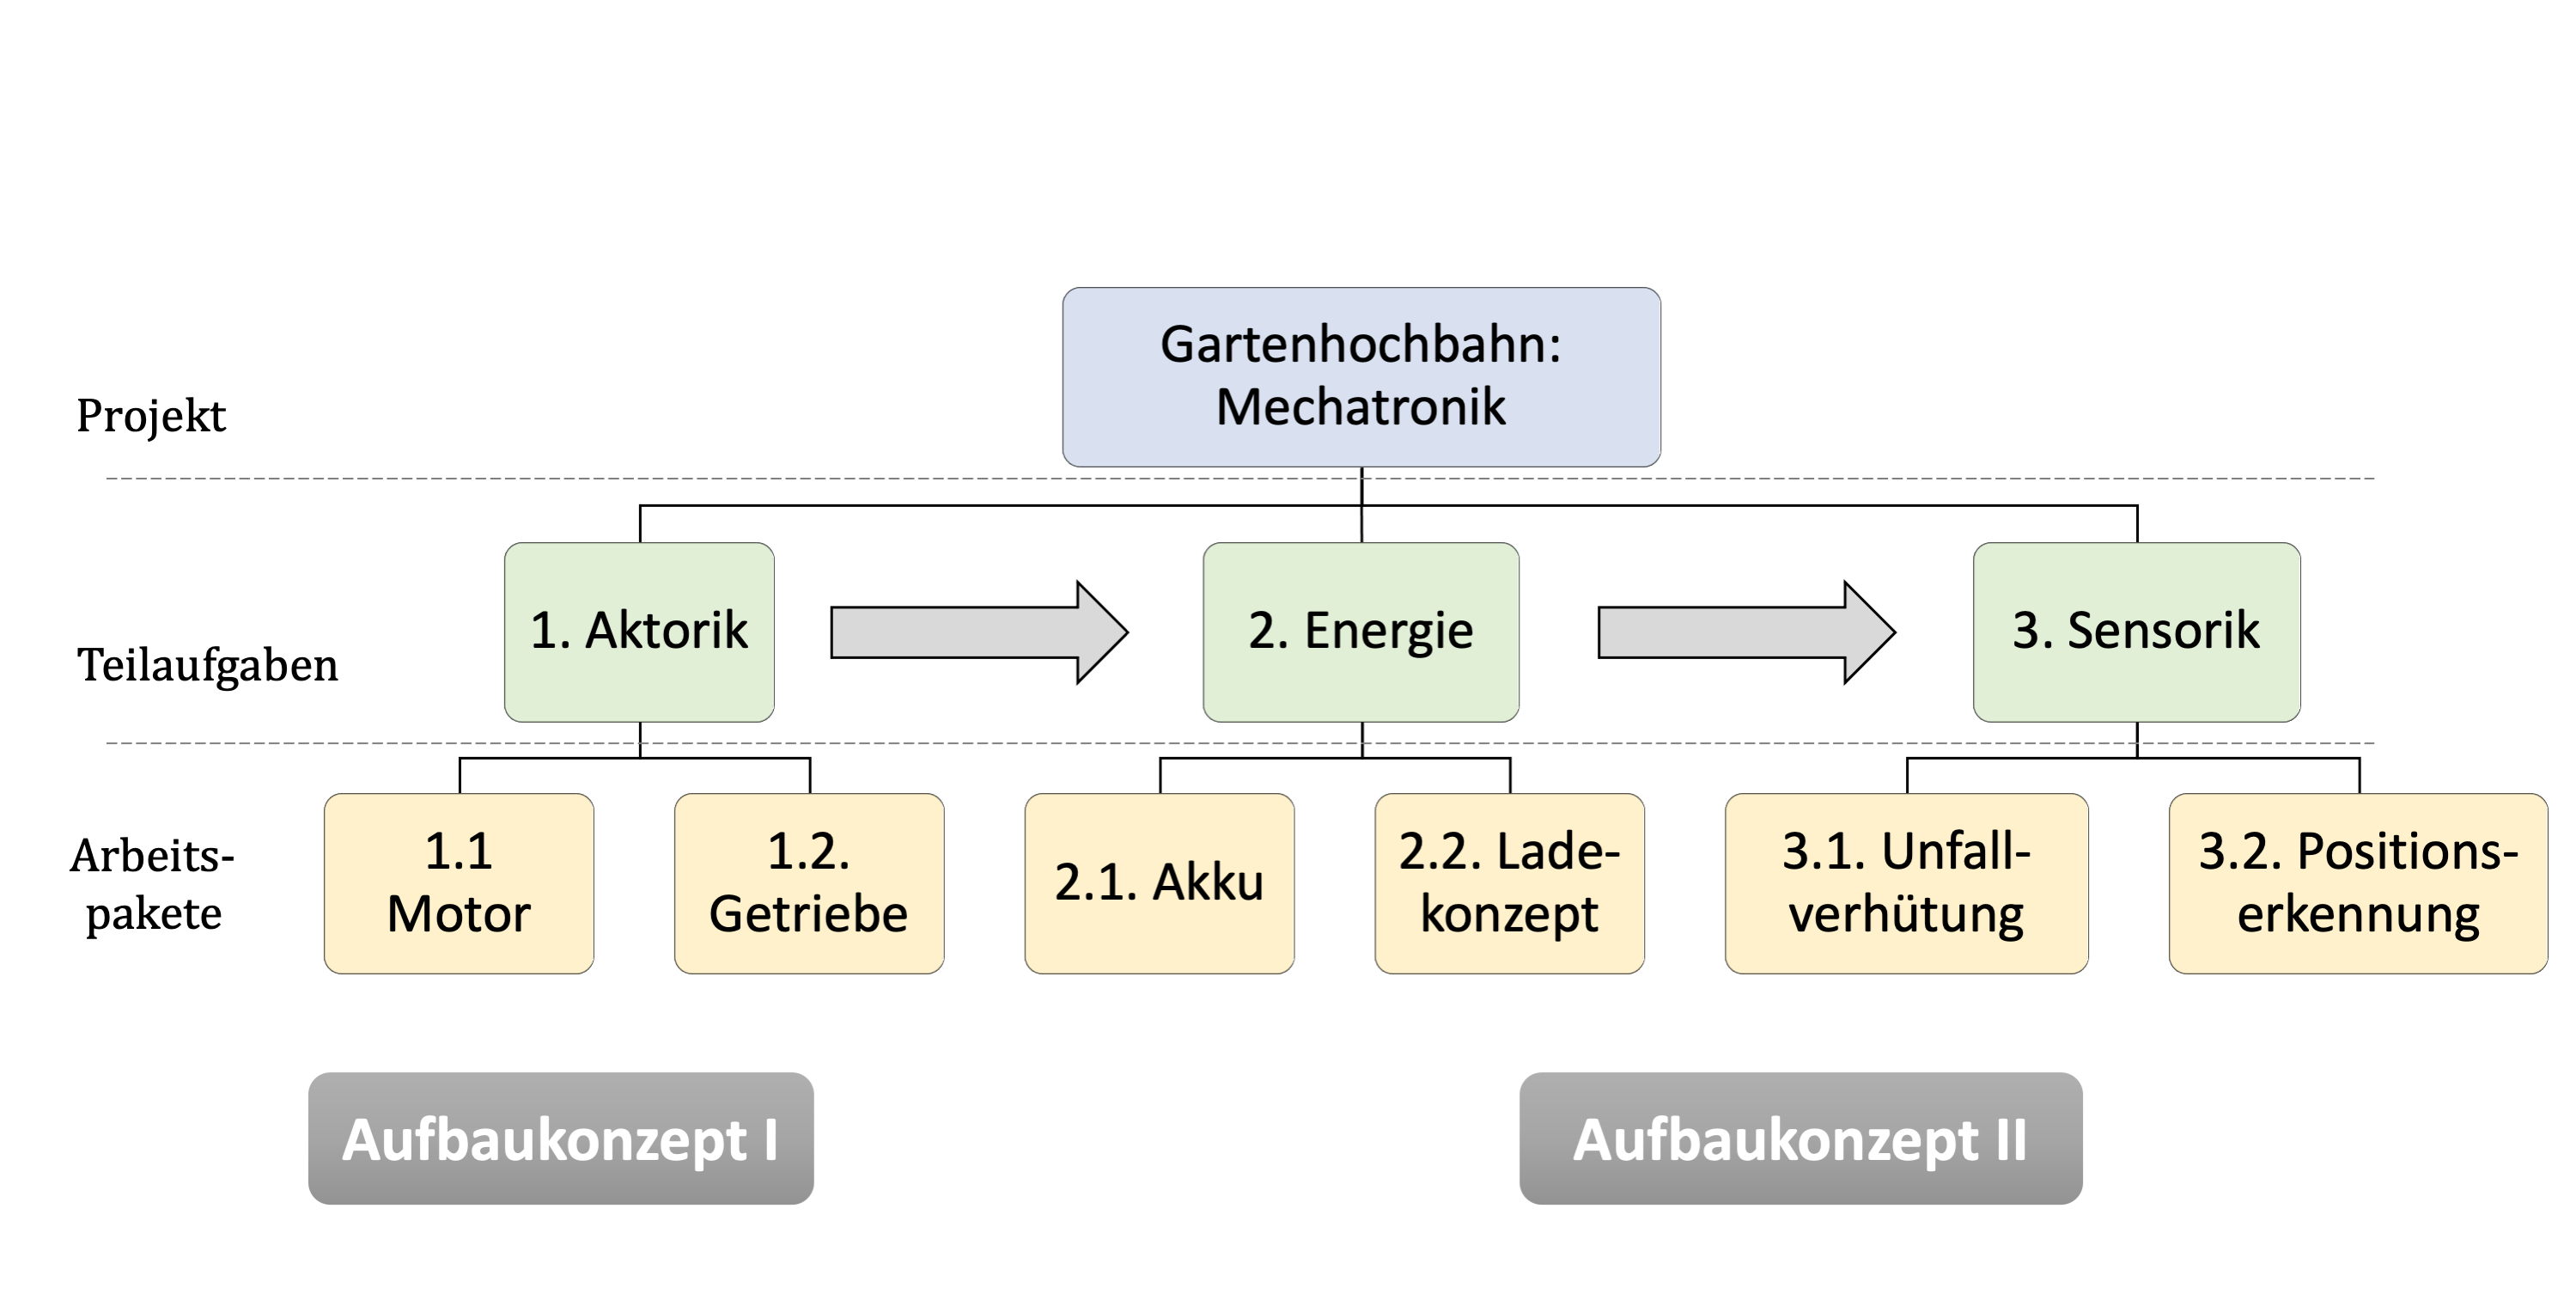
\includegraphics[width=17cm]{structure_mech.png}
		\caption{Projektstrukturplan mechatronischer Komponenten}
		\label{pic:structure_mech}
	\end{center}
\end{figure}

In \autoref{pic:structure_mech} ist der  Projektstrukturplan mit den mechatronischen Komponenten dargestellt. 
Das Projekt ist unterglieder in drei Telaufgaben. Diese werden in der nächsten Ebene in Arbeitspakete untergliedert. 
Da die Bereiche aufeinander aufbauend sind, können Zusammenhänge analysiert werden. In dem Schaubild sind die Bereiche entsprechend der zeitlichen Abfolge aufgetragen. Dementsprechend soll in einem ersten Schritt die Aktorik konzeptioniert werden. Dazu zählt die elektrische und mechanische Komponente des Antriebs. Dieser erste Entwurf des Antriebs wird im Aufbaukonzept I festgehalten. Mit den elektrischen Leistungsdaten der Aktorik wird im nächten Schritt das Energiekonzept ausgearbeitet. Auf diesen Bereich baut final die Konzeptionierungsphase der Sensorik auf. \\ 
Durch weitere Anforderungen aus den Bereichen Energie und Sensorik folgt das Aufbaukonzept II. 

\subsection{Projektablaufplan} %Wird noch schön eingefügt, fürs Testat reichts erst mal. 
%Werden auch in einem zweiten Schritt diene Aufgaben einfügen. 
\begin{figure}[t]
	\begin{center}
		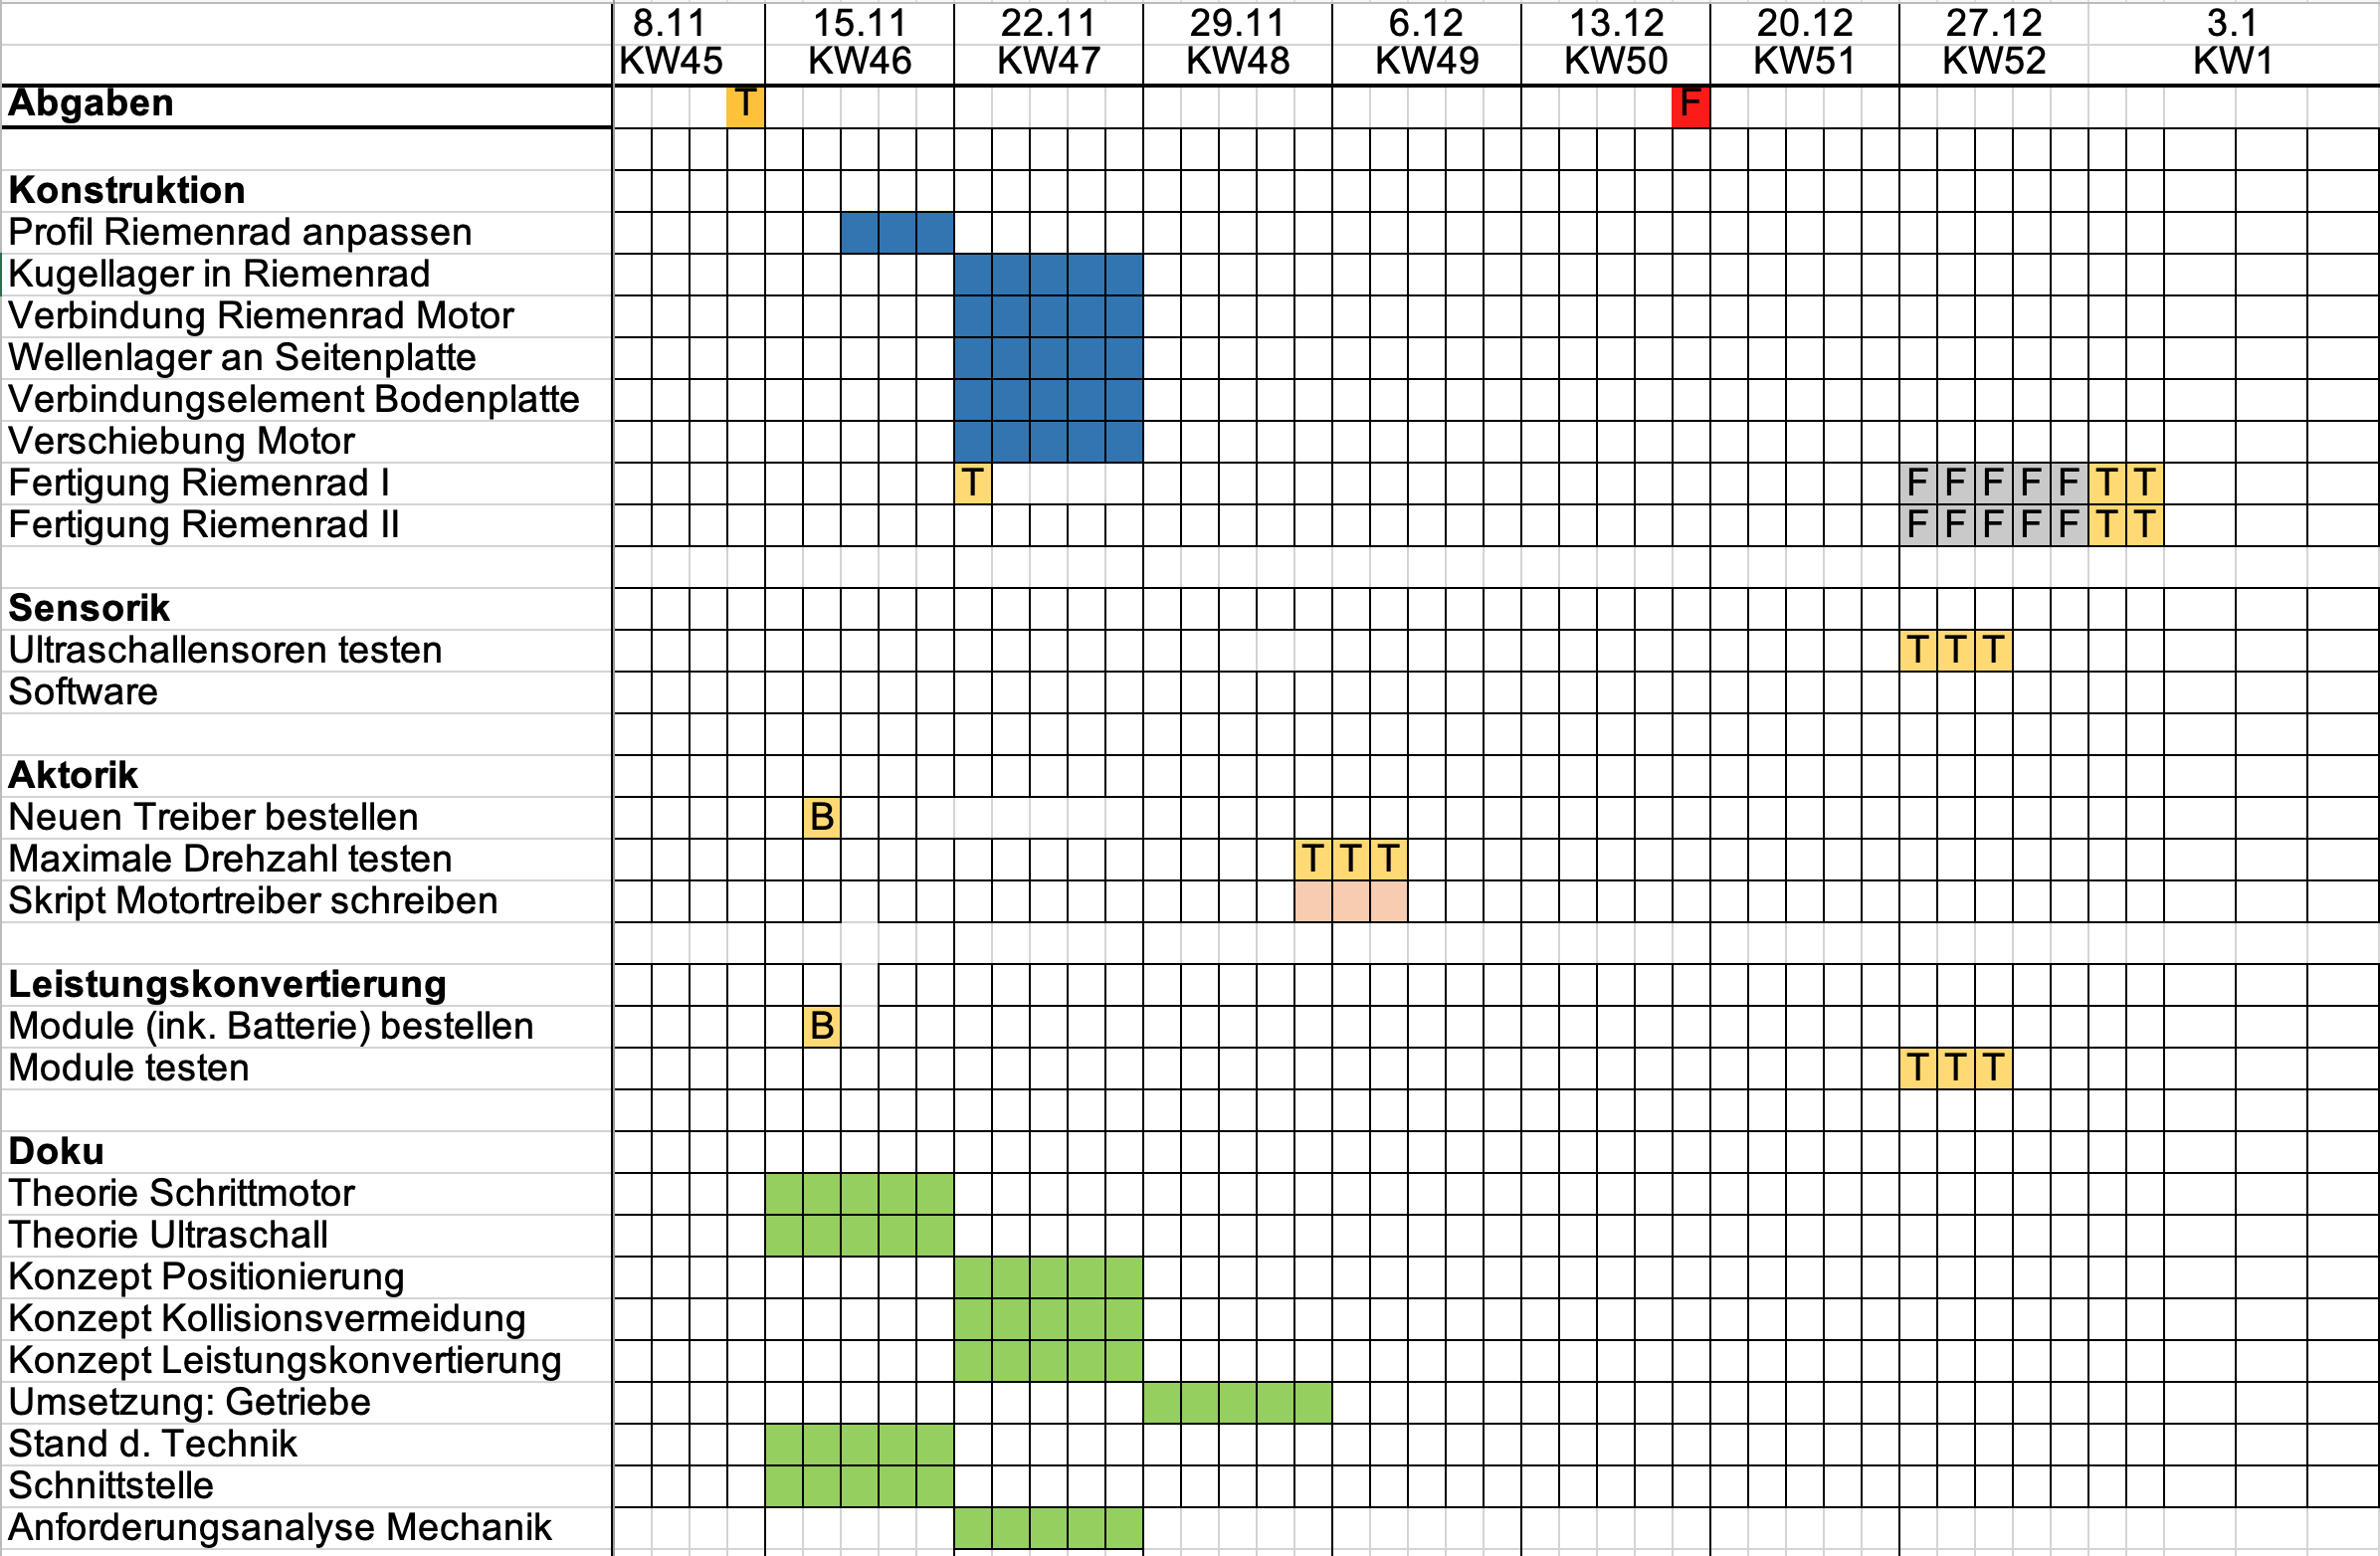
\includegraphics[width=17cm]{roadmap.png}
		\caption{Projaktablaufplan mechatronischer Komponenten}
		\label{pic:roadmap}
	\end{center}
\end{figure}


\chapter{Konzept}

Kukuk, hier ist ein Test, ob das mit dem Kompilieren auch funktioniert ;) 
\section{Mechanik}
\section{Hardware}
\subsection{Platine}
\subsection{Stromversorgung}
\subsection{Positionserkennung}

\section{Software}
Es gibt in diesem Projekt zwei Hauptsoftwarekomponenten, welche die Anlage steuern: Der Server, welcher Anfragen und Befehle an die Bahn verwaltet und die Bahn selbst,
welche für die Steuerung der Hardware zuständig ist. Der Server soll im Heimnetzwerk über die Adresse des Hosting-System erreichbar sein. Befehle an die Hochbahn sollen drahtlos mit \acrshort{mqtt} übertragen werden.
Auf der Bahn kommuniziert ein Arduino über einen ESP8266 mit dem Server und steuert gleichzeitig die Bahn. In den folgeneden Abschnitten wird die Konzeption dieser einzelnen Softwareteilen erläutert.

\subsection{Web-Applikation}
Die Web-Applikation bezeichnet die Benutzeroberfläche, welche sowohl in der Küche zum Einsehen von Bestellungen, als auch von Gästen zum Bestellen und Steuern der Bahn verwendet wird. Jeder Gast soll sich ein Konto erstellen und dabei seine Lieblingsfarbe auswählen können.
Bestellt dieser etwas kann so die Hochbahn in der individuellen Farbe leuchten. Dies dient zum einen der Freude der Gäste und zum anderen zum Erkennen, für wen die Bestellung ist. Angemeldet soll ein Nutzer über ein Menü unter folgenden Optionen
wählen können:
\begin{itemize}
	\item Allgemeines
	\item Mein Konto
	\item Bestellen
	\item Steuern
	\item Live-Verfolgung
\end{itemize}
Unter \textit{Allgemeines} werden generelle Infos zur Hochbahn angezeigt. Kontoeinstellungen wie Änderung der E-Mail Adresse oder Lieblingsfarbe werden unter \textit{Mein Konto} getätigt. Unter \textit{Bestellen} kann gewählt werden, was bestellt werden soll.
Ebenfalls ist dabei anzugeben, wohin die Bahn das bestellte fahren soll. Unter \textit{Steuern} kann die Bahn ohne eine Bestellung zu gewünschten Positionen gefahren werden. Die aktuelle Position und ggf. Bestellung kann unter \textit{Live-Verfolgung} eingesehen werden.
\subsection{Server}
\subsection{Client}
\subsection{Steuerung und Positionserkennung}

\chapter{Umsetzung}

\lipsum